
Once the plane-wave expansions are formed for each of the FGT boxes, step (ii)
involves translating the information to its interaction list to obtain the
local expansions. A direct scheme forms the local expansions by simply visiting
all the boxes in $\mathcal{I}|B|$ for each box $B$ and translating the wave
expansions according to (\ref{e:w2l}). Since the size of the interaction list
is $K^d$, this algorithm requires $\mathcal{O}(K^dp^d|B|)$ work to form all
local expansions, where $|B|$ is the total number of boxes. By using the
sweeping algorithm proposed in \cite{fggt}, the complexity of this step can be
reduced to $\mathcal{O}(3dp^d|B|)$. This algorithm is optimal in terms of work,
but is not ideal in terms of storage. In cases where we have non-uniform
distributions (resulting in several empty boxes), the sweep algorithm requires
storage at all boxes $B_i$, till the sweeps in all $d$ dimensions are
completed. We propose a new algorithm for accelerating the plane-wave
translations, which only needs $\mathcal{O}(|B|^\frac{d-1}{d})$ storage instead
of $\mathcal{O}(|B|)$ storage as required by the sweeping algorithm from
\cite{fggt}. 
% NOT CORRECT ...
% In addition, the algorithm is work optimal for distributions with \ul{distribution density} less than $60\%$ (for $d=3$).

\subsection{Accelerating the plane-wave translation step} Instead of sweeping
along each dimension one-by-one as with the method proposed in \cite{fggt}, our
algorithm visits each box only once and computes the full plane-wave
translation based on its neighbours which have already been visited. The
plane-wave expansions at a box $B_i$ can be represented as a combination of the
plane-wave expansions of its $2^{d} -1$ neighbours, along with corrections for
$2^d$ boxes. This results in an overall complexity of the sweep algorithm as
$\mathcal{O}((2^{d+1} -1)p^d|B|)$. The constant in the
complexity for this step increases from $3d\rightarrow2^{d+1} - 1$, which is
from $6\rightarrow7$ for $d=2$ and from $9\rightarrow15$ for $d=3$. 

The algorithm is illustrated in Figure \ref{fig:w2l}. The steps involved in the
algorithm are as follows, 
\begin{itemize} 
  \item First compute the local expansions at the outermost layer of the FGT
    boxes. Full computation ($K^dp^d$) is only required for the first box, as
    the local expansions for the other boxes can be computed by adding and
    subtracting layers from the expansions of the already computed boxes. 
  
  \item We propagate the local expansions from this initial layer to subsequent
    layers. Consider the case shown in Figure \ref{fig:w2l} where we need to
    compute the local expansion of the Green box ( $B(i+1,j+1)$), given the
    local expansions of the adjacent boxes (in Orange).  
  
  \item The local expansion $v_k^{B(i+1, j+1)}$ can be written in terms for the
    local expansions of the $2^d -1$ neighbours $B(i,j), B(i+1,j)$ and
    $B(i,j+1)$, along with corrections terms from the $2^d$ corners.
    These are marked in Figure \ref{fig:w2l} assuming $K=3, n=1$. 
    The local expansion is given by, 
    \begin{eqnarray*} 
    v_k^{i+1,j+1} &=& \sum_{\eta_{i,j} = 0,1} (-1)^{1 + d + |\eta|_1} e^{iz_k\eta s/\sqrt{\delta}} v_k^{i+\eta_i, j+\eta_j} \\
    & +& \sum_{\eta_{i,j}= 0,1} (-1)^{1 + d + |\eta|_1} e^{iz_k\eta ns/\sqrt{\delta}} w_k^{i+\eta_i, j+\eta_j}.
    \end{eqnarray*}
    
 %   e^{iz_k s/\sqrt{\delta}} v_k^{i+1,j} + e^{iz_k s/\sqrt{\delta}} v_k^{i,j+1} - e^{iz_k s/\sqrt{\delta}} v_k^{i,j} - e^{iz_k ns/\sqrt{\delta}} w_k^{i+n+1,j+n+1} + e^{-iz_k ns/\sqrt{\delta}} w_k^{i-n,j-n}
  
  \item The propagation can then be used to propagate to the remaining boxes in
    the new propagation layer. At any given stage only the values of the
    propagation layer needs to be stored. The values of any non-zero FGT boxes
    doesn't need to be remembered.

\end{itemize}


%\begin{figure}[h]
%\centering
%\begin{tikzpicture}
%	
%	\draw[fill=orange!10] (0,0) rectangle +(8,2);
%	\draw[fill=orange!10] (0,2) rectangle +(2,6);
%		
%	% the grid ...
%	\draw[step=2cm] (0,0) grid (8,8);	
%	
%\end{tikzpicture}
%\caption{\small The outermost layer, for which the local expansions are computed directly. 
%}
%\label{fig:outer}
%\end{figure}

\begin{figure}[h]
\centering
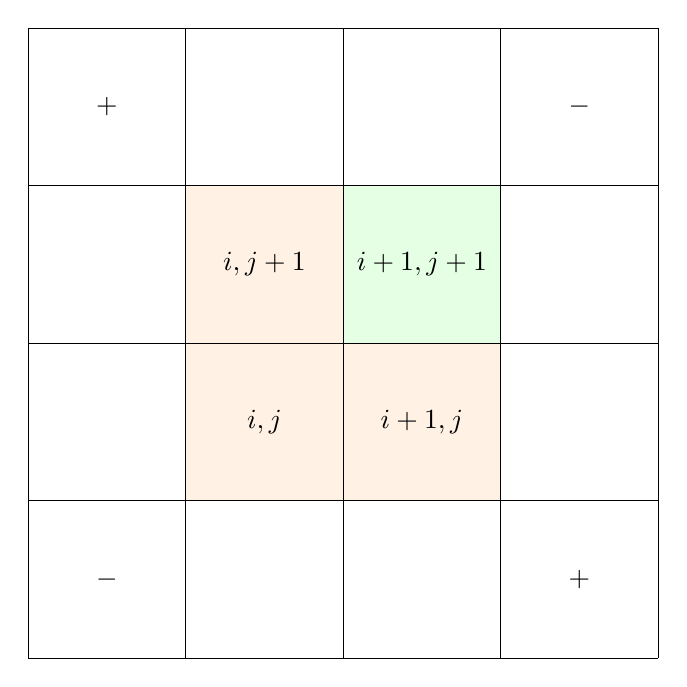
\begin{tikzpicture}
	
	\draw[fill=orange!10] (2,2) rectangle +(4,2);
	\draw[fill=orange!10] (2,2) rectangle +(2,4);
	
	\draw[fill=green!10] (4,4) rectangle +(2,2);		
	% the grid ...
	\draw[step=2cm] (0,0) grid (8,8);	
	
	\draw (3,3) node {$i, j$};
	\draw (5,3) node {$i+1, j$};
	\draw (3,5) node {$i, j+1$};
	\draw (5,5) node {$i+1, j+1$};
	
	\draw (1,1) node {$-$};
	\draw (7,7) node {$-$};
	\draw (1,7) node {$+$};
	\draw (7,1) node {$+$};
			
\end{tikzpicture}
\caption{\small The propagation of the local expansions using neighbors. 
}
\label{fig:w2l}
\end{figure}


